\begin{figure}[h!]
    \centering
    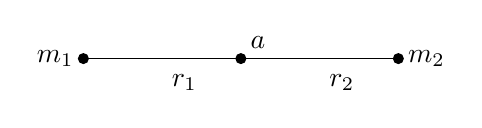
\begin{tikzpicture}
        \draw 
            (-2,0)--(2,0);
        \fill
            (-2,0) circle[radius=2pt] node[anchor=east]{$m_{1}$};
        \fill
            (2,0) circle[radius=2pt]node[anchor=west]{$m_{2}$};
        \fill
            (0,0) circle[radius=2pt]node[anchor=south west]{$a$};
        \draw 
            (-1, -0.3) node[anchor=west]{$r_{1}$};
        \draw 
            (1, -0.3) node[anchor=west]{$r_{2}$};
    \end{tikzpicture}
    \caption{Crude depiction of two objects of mass $m_{1}$, $m_{2}$ orbiting around their common center of mass.}
    \label{fig:binaries}
\end{figure}